\chapter*{Introduction}\addcontentsline{toc}{chapter}{Introduction}
Amidst the countless stars and galaxies we observe in the Universe lie 
undetected structures of dark matter, orders of magnitude larger than 
the luminous objects they engulf. These vast invisible structures began 
in the very early Universe, as quantum fluctuations in the aftermath of 
the Big Bang. 
%These vast invisible structures began as quantum fluctuations in the beginning of the Universe in the aftermath of the Big Bang. 
During the subsequent period of inflation (\todo{cite?}), these primordial fluctations 
were amplified by the accelerated expansion of the Universe and then 
propagated through gravitational instability for billions of years. 

Despite constituting most of the matter in the Universe, dark matter 
has yet to be directly observed. In fact, it can only be studied through 
its gravitational interactions with luminous baryons — the matter that 
constitutes stars, galaxies, and celestial objects that emit light. 
In a way, the galaxies we observe in the cosmic volumes probed by our 
telescopes act as illuminated beacons tracing the vast dark matter 
terrains of the Universe.

Over the past decade, spectroscopic redshift surveys like the 
Baryon Oscillation Spectroscopic Survey (BOSS\todo{cite}) have 
exploited these galactic beacons to map out the cosmic structure
of the Universe. Precise measurements of distance and growth 
of large-scale structure (LSS) from these surveys, provide tests 
of cosmological models that desribe the content, geometry and history 
of the Universe. \todo{By analyzing measurements of LSS,}


Through these galaxies, we can explore the properties of the underlying dark matter
and the growth of their structure. Measurements that quantify these properties allow us to make
precise calculations of cosmological parameters, which quantify the content, geometry, and
expansion history of the Universe. Ultimately the constraints we measure on these parameters,
enlighten us on the properties of dark energy, which remains one of the most crucial unsolved
questions in cosmology. Certainly these precise cosmological measurements require a profound
understanding of the formation and evolution of galaxies. Unfortunately there is no clear
narrative of galaxy formation and evolution due to the complex, non-linear, and stochastic nature
of the physical processes that govern them.

In fact, galaxy formation and evolution remain another central unsolved questions in
astrophysics and cosmology. However, since galaxies are enveloped in the massive gravitational
wells of their host dark matter structures, the underlying dark matter of galaxies undoubtedly
plays a crucial role in their formation and evolution. Therefore, with its implications on the most
crucial questions in both cosmology and our understanding of galaxies, the interactions between
galaxies and their host dark matter environments pose some of the most impactful questions,
questions that I seek to answer in my dissertation. 


%\section{$\Lambda$CDM cosmology}
\section{Large Scale Structure}
From the early Universe, primordial quantum fluctuations grow into the 
large-scale structures of the Universe we observe today through the different
epochs of cosmic history and by gravitational instability. In this section, I briefly 
describe the simplified ({\em linear}) theory of this evolution and explain core 
concepts of LSS cosmology using galaxies. Lets begin by defining the matter 
overdensity field (or density fluctuation) at comoving position ${\bf r}$: 
\beq \label{eq:delta}
\delta({\bf r}) = \frac{\rho({\bf r}) - \bar{\rho}}{\bar{\rho}}, 
\eeq
where $\rho({\bf r})$ and $\bar{\rho}$ are the density field and mean 
density respectively. In Fourier space ($k$-space), Eq.~\ref{eq:delta} can 
be Fourier transformed, 
\beq
\delta({\bf k}) = \int \frac{{\rm d^3}{\bf r}}{(2\pi)^3} e^{-i{\bf k}\dot{\bf r}}\;\delta({\bf r}).
\eeq
For describing the evolution of the overdensity field, Fourier space is generally 
favored over configuration space because, as derived later in the section,
the Fourier modes of $\delta$ evolve independently in linear theory -- 
\emph{i.e.} on large scales.

The information in the overdensity field is often quantified using its 
$N$-point statistics (\todo{cite Peebles bernardeua}). In fact, the two-point
statistic is one of commonly used tool in large scale structure studies.
This two-point statistic (also referred to as the correlation function) is
defined as, 
\beq
\xi(r) = <\delta({\bf x})\delta({\bf x} +  {\bf r})>
\eeq
and in Fourier space as,
\beq
<\delta({\bf k})\delta({\bf k'})> = (2\pi)^3 P(k) \delta^{D}({\bf k}+{\bf k'}).
\eeq
$\delta^{D}$ is the Dirac delta function and $P(k)$ is the {\em powerspectrum}, 
the Fourier transform of $\xi$. In principle, $\xi$ and $P(k)$ contain the same 
information. In practice, however, analyzing $\xi$ versus $P(k)$ carry different 
caveats (\todo{cite FKP}). Throughout this section, and also the dissertation, 
I will mainly focus on the powerspectrum. 

The evolution of the dark matter overdensity field can be derived (on 
sub-horizon scales) as follows. For pressureless dark matter, the equation of motion
can be derived from the continuity, Euler, and Poisson equations
\beqa 
\frac{\partial \rho}{\partial t} + \nabla \dot \rho {\bf u} = 0  \\ 
\frac{\partial {\bf u}}{\partial t} + ({\bf u} \dot \nabla) \dot {\bf u} - \nabla\Phi = 0 \\ 
\nabla^2\Phi - 4 \pi G \rho = 0 
\eeqa
to 
\beq \label{eq:meszaros}
\frac{\partial^2 \delta}{\partial t^2} + 2 \frac{\dot{a}}{a} \frac{\partial \delta}{\partial t} - 4 \pi G \bar{\rho} \delta = 0.
\eeq
${\bf u}$ is the velocity field, $\Phi$ is the gravitational potential, and $a$ 
is the scale factor. For a detailed derivation I refer readers to \todo{cite Peebles 
or Dodelson}. Eq.~\ref{eq:meszaros} a second order differential equation, therefore,
the solution can be written as 
\beq 
\delta({\bf r}, t) = D^{(+)}(t) A({\bf r}) + D^{(-)}(t) B({\bf r}).
\eeq
The density flucation has two components: a growing mode $D^{(+)}$ and a decaying 
mode $D^{(-)}$. The decaying mode decreases with time and its contribution becomes negligible
leaving only the growing mode in the late Universe. Now in order to quantify
the evolution of the growing mode $D^{(+)}$, one commonly used quantity is the 
``growth rate of structure'': 
\beq
f = \frac{ d {\rm ln}\;D^{(+)}}{d {\rm ln}\;a}. 
\eeq
This growth rate of structure is a key quantity in LSS cosmology for testing different 
cosmological models and theories of gravity. $f$ will be discussed further in Section~\ref{sec:rsd}.

From the early Universe the density fluctuations evolve through different epochs in 
cosmic history: inflation, radiation-dominated, and matter-dominated eras. Each of 
these periods leave an imprint on the evolution of $\delta$. Fig.~\ref{fig:lifo}, 
marks the different eras in the early Universe and plots how the physical scale of 
the Universe, represented by the Hubble radius, evolves with $a$. 

During inflation, the Hubble radius remains constant. Afterwards the Universe 
becomes radiation dominated. Based on the Friedmann equations the Hubble radius 
during the radiation dominated era is approximately $\propto a^{2}$. The Universe then 
becomes matter dominated and the Hubble radius is approximately $\propto a^{3/2}$. 
Meanwhile, the physical scale of perturbations is 
$\lambda_{phys} = \lambda_{comov}\ a(t) \propto a(t)$. As Fig.~\ref{fig:lifo} 
illustrates, perturbations exit the Hubble radius during inflation then 
reenter the Hubble radius later on. Depending on the physical scale of the 
perturbation, it can enter either during the radiation dominated  
(smaller scale) or matter dominated (larger scale) era. 


The physical scale of perturbations that enter the horizon at the time of 
matter-radiation equality ($a(t) = a_{eq}$), $\lambda_{eq}$ is $\sim 500 h^{-1}Mpc$.
The perturbations that enter before the matter-radiation equality during 
the radiation dominated era, have physical scales $\lambda_{phys} < \lambda_{eq}$. 
These smaller scale perturbations, todo{explain the supression} 
On the other side, the larger scale perturbations with $\lambda_{phys} > \lambda_{eq}$
enter after matter-radiation equality during the matter dominated epoch. These 
perturbations do {\em not} experience the suppression of growth of the radiation 
dominated era. Therefore, as the overdensity field goes through these epochs, its 
growth on small scale is suppressed by a factor of $\sim k^4$.  


In practice, this scale dependent evolution of the density fluctuation is 
quantified through the ``transfer function'' $T(k)$ (\todo{cite all the transfer function papers}). After inflation the 
powerspectrum of the density fluctation can be summarized by: 
\beq
P_{inf}(k) \propto k^{n_s}
\eeq
where $n_s \sim 1$ \todo{cite inflation papers: Harrison (1970), Zel’dovich (1972) and Peebles Yu (1970) Komatsu et al. 2011}. Then powerspectrum of the density 
fluctuation in the late Universe can be expressed as 
\beq
P(k) \propto k^{n_s} T^2(k) D^2(k). 
\eeq
$D(k) \equiv D^(+)$ from earlier this section. 

\begin{figure*}
\begin{center}
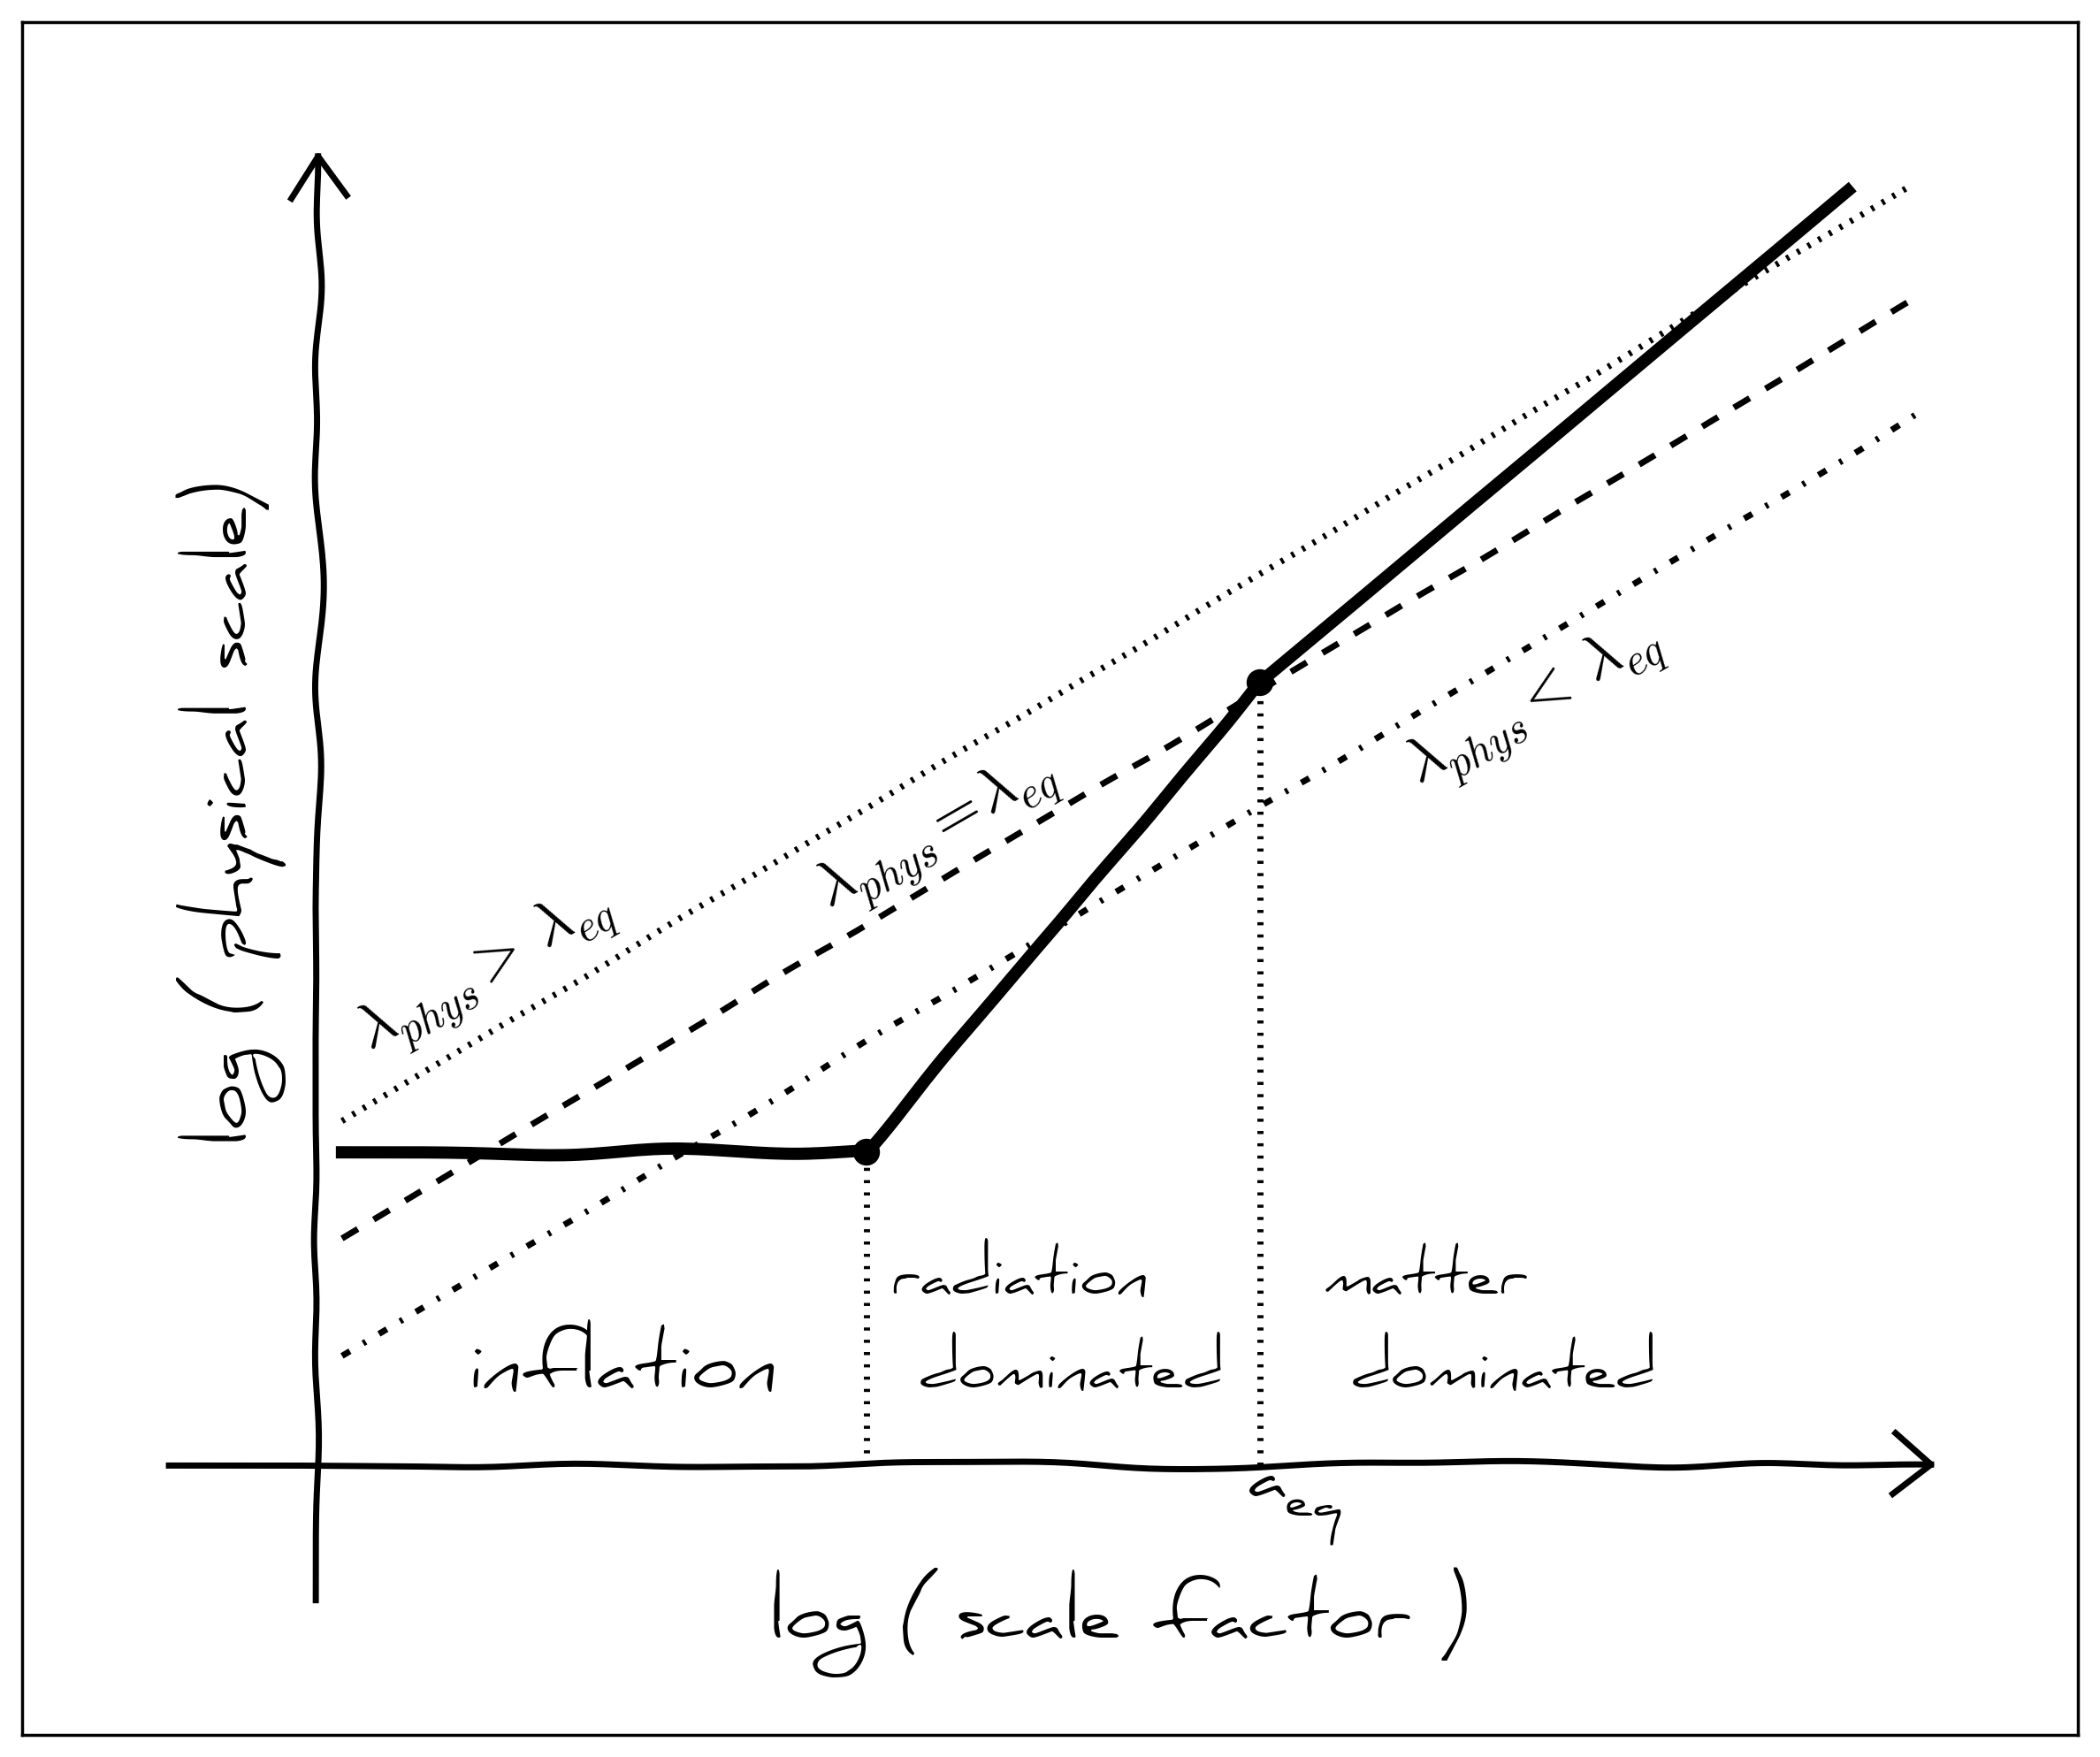
\includegraphics[width=\textwidth]{figs/lifo.png}
\caption{Schematic diagram that illustrates the evolution of the Hubble radius
(Above) The evolution of the Hubble radius (solid line) during inflation (flat), radiation
domination, and matter domination (note inflection). Dashed, dotted, and dot-dashed
lines show the physical length of three constant comoving scales. The scale corresponding
to the current Hubble radius cH−1
0 first “left the horizon” about 60 e-folds before the end
of inflation (open circle).
} \label{fig:lifo}
\end{center}
\end{figure*}

\todo{paragraph about how because D and T depend on cosmological parameters 
    so powerspectrum measurements of the matter density fluctuation can be 
    used a tests of the cosmological models.
}
So powerspectrum measurements of the matter density fluctuations can be compared
to predictions of various cosmological models in order to produce constraints 
on cosmological parameters, better understand dark energy, and test theories of 
gravity. Unfortunately, most of the matter in the Universe is in the form of dark 
matter and does not interact with radiation. 

Observers cannot measure the spatial statistics (or clustering) of dark matter 
directly. Instead, we measure the clustering of galaxies and quasars, which trace
the underlying matter distribution. The smoothed galaxy/quasar density field is 
approximated by a local function of the matter density field
\beq
\delta_g({\bf r}) = F( \delta({\bf r} ). 
\eeq
This function can then be expanded Taylor series,
\beq
\delta_g({\bf r}) = \sum\limits_{k=0}^{\infty} \frac{b_k}{k!} \delta^k. 
\eeq
$b_1$ is referred to as the linear bias factor and $b_0$ is chosen so that
$<\delta_g> = 0$. To linear order, 
\beq
P_g(k) = b_1^2 P(k). 
\eeq
For galaxies, $b_1 > 1$ (\todo{cite Zehavi 2005, Sheldon 2009, Gastanage 2009}). 
Galaxies are {\em biased} tracers of the matter distribution because luminous galaxies
reside in larger potential wells and more massive overdensities have stronger
clustering properties than than less massive ones (\todo{manera 2010}). 
%indicating brighter objects reside in larger potential wells, as there was more infall of gas. N−body simulation analyses find that larger dark matter halos have stronger clustering properties than less massive

\todo{insert transition to redshift space distortions here} 

\section{Redshift-Space Distortions} \label{sec:rsd}
Spectroscopic redshift surveys such as BOSS catalog the angular positions (right ascension 
and declination) and redshifts of galaxies in the sky. 

\beq
z_{obv} = z_{true} +  \frac{v_{pec}}{c}
\eeq

Kaiser Effect
\beq
\delta^{(s)}({\bf k}) = (1 + f \mu_k^2) \delta({bf k})
\eeq
\beq
\delta_g^{(s)}({\bf k}) = (b + f \mu_k^2) \delta({bf k})
\eeq
\beq
P_g^{(s)}(k) = (b + f \mu_k^2)^2 P(k)
\eeq

\beq
\mu = \hat{z} \odot \hat{k} 
\eeq

Fingers of God 
\beq
P_g^{(s)}(k) = e^{-f^2 \sigma_v^2 \mu^2 k^2} (b + f \mu^2)^2 P(k)
\eeq

% redshift space distorted p(k)
% bispectrum intro
% brief neutrino mass  


Redshifts measure both the velocity due to cosmic expansion and the peculiar velocities driven by gravitational attraction from LSS. 
The peculiar velocity component anisotropically ``distorts'' redshift-space galaxy clustering. 
Measuring this redshift-space distortion (RSD) allows us to infer the growth of structure, which we can then use to test GR and modified gravity scenarios. 
Galaxy clustering also provides a unique window to probe fundamental physics {\em i.e.} \mneut. 
Neutrinos suppress the growth of structure below their free-streaming scale and leave imprints on the LSS. 
From the imprints on galaxy clustering, we can place limits on \mneut. 

\section{Galaxy Clustering Analysis}%Galaxy-Halo Connection}

\begin{enumerate}
{\item 
multipole expansion, observables, etc
}
{\item 
standard likelihood analysis  
}
{\item 
limits of the current framework
}
{\item 
mention bispectrum
}
{\item 
mention chapters and how they improve things
}
\end{enumerate}

\chapname s~\chapalt{fc} and~\chapalt{galenv} have both been refereed and
published in the astronomical literature.
\chapname s~\chapalt{abc} and~\chapalt{galhalo} have been submitted to the 
\emph{Monthly Notices of the Royal Astronomical Society} and \emph{The Astrophysical Journal},
respectively, and updated in response to the referees' comments.
All of these \chapname s were co-authored with collaborators but the majority
of the work and writing in each \chapname\ is mine.
Below, I describe my contributions to each \chapname:
\begin{enumerate}

{\item 
For \chap{fc}, I developed the idea for the project in collaboration with Roman
Scoccimarro and Michael Blanton. I implemented the project with contributions 
from Roman Scoccimarro. The project utilized simulation data from Jeremy Tinker
and Sergio Rodr\'{i}guez-Torres. I wrote the paper with additions from 
Roman Scoccimarro and edits by Michael Blanton. 
}

{\item 
For \chap{abc}, I developed the idea for the project in collaboration with 
Mohammadjavad Vakili, Andrew Hearin, and David Hogg. I implemented the project 
with Mohammadjavad Vakili and contributions from Andrew Hearin and Kilian Walsh.
The project utilized software written by Andrew Hearin and Duncan Campell. 
I wrote the paper together with Mohammadjavad Vakili with additions from
Andrew Hearin, David Hogg, and Kilian Walsh.
}

{\item 
For \chap{galenv}, I developed the idea for the project in collaboration with 
Michael Blanton. I implemented the project using catalogs constructed by 
John Moustakas from observations made by the PRIMUS collaboration (Alison Coil,
Richard Cool, Daniel Eisenstein, Ramin Skibb, Kenneth Wong, and Guangtun Zhu).
I wrote the paper with additions from Michael Blanton. 
}

{\item 
For \chap{galhalo}, I developed the idea for the project in collaboration with 
Jeremy Tinker. I implemented the project using simulation data from Andrew 
Wetzel. I wrote the paper with comments and edits by Jeremy Tinker and Andrew 
Wetzel. 
}
\end{enumerate}



%Over the past few years, the field of extrasolar planet (exoplanet) research
%has really taken off thanks, in large part, to the exquisite time series
%photometry measured by the \kepler\ Mission \citep{Borucki:2010}.
%The Mission enabled the discovery of thousands of planets and planet
%candidates outside the Solar System \citep{Rowe:2015}.
%The zoo of planetary systems is extremely diverse---with sizes, masses, and
%orbital periods spanning orders of magnitude---and the statistics are now
%sufficient to test theories of planet formation and evolution.
%
%The \kepler\ Mission has changed the face of exoplanet research because of its
%photometric precision and the sheer volume of the dataset.
%In order to discover small planets that serendipitously transit their host
%stars, the \kepler\ spacecraft was designed to monitor the brightness of about
%150,000 stars in one $10^\circ \times 10^\circ$ patch of the sky nearly
%continuously---at a half-hour cadence---for more than three years with a
%relative precision of a few parts-per-million for the brightest stars.
%The Mission surpassed its fiducial goals and took data for over 4~years before
%two of the reaction wheels used to stabilize the pointing failed in the Spring
%of 2013.
%
%Despite the fact that most planets never transit their host star---based on
%geometric effects alone---and the fact that transit surveys are most sensitive
%to large planets on short orbits, the discoveries made in the \kepler\ dataset
%and careful characterization of the selection effects and search completeness
%have enabled detailed studies of the true underlying distribution of planets
%over a wide range in parameter space \citep[examples include][and
%\chap{exopop}]{Howard:2012, Petigura:2013, Foreman-Mackey:2014,
%Dressing:2015}.
%These observational studies of the population of exoplanets are arguably the
%ultimate goal of the \kepler\ Mission because they open the door to direct
%comparison with theories of planet formation and evolution.
%
%The different constraints on the intrinsic rate and distribution of planets
%differ in detail but several overarching results are solid.
%The evidence suggests that every cool M-star has at least one planet in orbit
%\citep{Dressing:2013, Dressing:2015} and more than half of the other main
%sequence stars should have planetary systems \citep{Howard:2012, Fressin:2013,
%Petigura:2013, Foreman-Mackey:2014}.
%Of these planets, the most intrinsically common are in the ``super-Earth'' or
%``mini-Neptune'' range from about twice to four-times the radius of Earth.
%A combination of radial velocity follow-up and hierarchical inference methods
%indicate that most of these mini-Neptunes gaseous instead of rocky
%\citep{Weiss:2014, Rogers:2015} but since there are no planets like this in
%the Solar System, understanding them is crucial to our theories of planetary
%system formation.
%
%% These results can be used as targets for numerical simulations of planetary
%% systems or population level inferences can be combined with theoretical models
%% to \citep{Wolfgang:2014, Rogers:2015}.
%
%One shortcoming of the \kepler\ Mission was that it only targeted one field
%and in that frame, the main focus was on relatively faint F, G, and K dwarf
%stars.
%This target selection was chosen to enable the study of long-period planets
%and the discovery of Earth-sized planets orbiting Sun-like stars.
%Unfortunately many of these stars and their planetary systems are not amenable
%to radial velocity follow-up because the star is too faint to achieve the
%required velocity precision or the expected velocity amplitude is too small to
%detect.
%In the Summer of 2014, the \kepler\ instrument was re-purposed and it began
%taking data in a mode called \KT\ with substantial degraded pointing accuracy
%\citep{Howell:2014}.
%Because of technical constraints, \KT\ targets a different field in the
%ecliptic plane every three months.
%This means that it can target stars in different environments and focus on
%gathering the census of planets orbiting bright, nearby stars.
%It has been demonstrated that the data from \KT\ can reach precisions
%comparable to the original Mission and that it can be used to discover
%transiting exoplanets \citep[][and \chap{ketu}]{Vanderburg:2014,
%Vanderburg:2015, Crossfield:2015, Foreman-Mackey:2015}.
%The discoveries made using \KT---and the upcoming \tess\ Mission---improve our
%knowledge of the population of exoplanets, especially those planets that orbit
%the cool M-stars that were not prioritized by the \kepler\ Mission.
%These discoveries also present excellent targets for radial velocity follow-up
%and even spectroscopic observations of their atmospheres using the planned
%\project{James Webb Space Telescope}.
%
%The technical problem of searching for transits in the massive datasets
%produced by a time series mission like \kepler\ is a hard one.
%The relative change in brightness caused by the transit of planet in front of
%its host star is given by the area ratio between the planet and star
%\citep{Winn:2010}.
%Therefore, when an Earth-sized planet transits a Sun-like star, the amplitude
%of the signal is smaller than 100 parts-per-million.
%What's more, in the case of the Earth's orbit, this signal would only last for
%a little over half a day, once every year.
%Add to this the fact that most light curves are fraught with signals induced
%by stellar variability \citep{Basri:2013}, spot activity
%\citep{McQuillan:2014}, and instrumental effects \citep{Stumpe:2012,
%Smith:2012} with amplitudes far exceeding most transits.
%In order to find transits, we must, therefore, develop methods for efficiently
%and robustly mining large sets of light curves for tiny, sparse signals.
%Nearly all transit search algorithms rely on some sort of matched filter that
%is made insensitive to noise by pre-processing the light curves to remove the
%trends or by designing an estimator that is insensitive to these effects
%\citep[][]{Kovacs:2002, Kovacs:2005, Berta:2012, Petigura:2013,
%Foreman-Mackey:2015}.
%
%Despite the attempts made to develop search algorithms that are robust to
%systematics and variability, all automated search results are completely
%dominated by false signals induced by poorly characterized noise in the light
%curves.
%In practice, automatic removal of these events has not been demonstrated to be
%sufficient---although the results are starting to look promising
%\citep{Jenkins:2014}---and all published catalogs of planet candidates are
%manually vetted.
%This means that the published list of candidates is \emph{chosen by a
%person---or group of people---going through the data by hand}.
%This method is not efficient or scalable so a substantial set of heuristic
%filtering is applied to the candidate list even before anyone looks at the
%light curves.
%One of the standard filters is to only consider candidates with at least three
%observed transits \citep[for example][]{Petigura:2013, Burke:2014, Rowe:2015}.
%This greatly restricts the range of parameter space that can be search.
%In particular, these methods will miss any planets on orbits longer than a
%fraction of the survey baseline.
%
%While transit surveys present the most effective means for systematic
%exoplanet characterization, their use is limited by existing transit search
%methodologies for planets with long orbital periods.
%In many cases, massive long-period planets dominate the dynamics of the
%planetary systems---like Jupiter in the Solar System---but their existence is
%completely missed by \kepler.
%This shortcoming becomes even more severe for \KT\ and \tess, transit surveys
%with shorter baselines.
%The final \chapname\ of this dissertation presents a novel method for transit
%search designed specifically to discover and quantify these important planets.
%
%The study of exoplanets and their population has been driven by the public
%\kepler\ dataset and, in particular, by methods and software solutions
%developed by graduate students and young researchers around the world to
%squeeze all the available information out of the existing dataset.
%This dissertation presents methods developed with exactly these goals in mind.
%Each \chapname\ is accompanied by an open source implementation of the method
%and code to reproduce the results and figures.
%Of these projects, the most popular is the Markov Chain Monte Carlo
%implementation \project{emcee} \citep[][and
%\chap{emcee}]{Foreman-Mackey:2013}.
%With nearly 300 citations at the time of
%writing\footnote{\url{http://adsabs.harvard.edu/cgi-bin/nph-ref_query?bibcode=2013PASP..125..306F&amp;refs=CITATIONS&amp;db_key=AST}}
%and an active community on
%\project{GitHub}\footnote{\url{https://github.com/dfm/emcee}}, \project{emcee}
%has enabled many modest and ambitious probabilistic inferences across
%astrophysics.
